\documentclass{beamer}
\usepackage[utf8]{inputenc}

\usetheme{Madrid}
\usecolortheme{default}
\usepackage{amsmath,amssymb,amsfonts,amsthm}
\usepackage{txfonts}
\usepackage{tkz-euclide}
\usepackage{listings}
\usepackage{adjustbox}
\usepackage{array}
\usepackage{tabularx}
\usepackage{gvv}
\usepackage{lmodern}
\usepackage{circuitikz}
\usepackage{tikz}
\usepackage{graphicx}

\setbeamertemplate{page number in head/foot}[totalframenumber]

\usepackage{tcolorbox}
\tcbuselibrary{minted,breakable,xparse,skins}



\definecolor{bg}{gray}{0.95}
\DeclareTCBListing{mintedbox}{O{}m!O{}}{%
  breakable=true,
  listing engine=minted,
  listing only,
  minted language=#2,
  minted style=default,
  minted options={%
    linenos,
    gobble=0,
    breaklines=true,
    breakafter=,,
    fontsize=\small,
    numbersep=8pt,
    #1},
  boxsep=0pt,
  left skip=0pt,
  right skip=0pt,
  left=25pt,
  right=0pt,
  top=3pt,
  bottom=3pt,
  arc=5pt,
  leftrule=0pt,
  rightrule=0pt,
  bottomrule=2pt,
  toprule=2pt,
  colback=bg,
  colframe=orange!70,
  enhanced,
  overlay={%
    \begin{tcbclipinterior}
    \fill[orange!20!white] (frame.south west) rectangle ([xshift=20pt]frame.north west);
    \end{tcbclipinterior}},
  #3,
}
\lstset{
    language=C,
    basicstyle=\ttfamily\small,
    keywordstyle=\color{blue},
    stringstyle=\color{orange},
    commentstyle=\color{green!60!black},
    numbers=left,
    numberstyle=\tiny\color{gray},
    breaklines=true,
    showstringspaces=false,
}
%------------------------------------------------------------

\title
{4.7.64}
\date{September 4,2025}
\author 
{AI25BTECH11003 - Bhavesh Gaikwad}



\begin{document}


\frame{\titlepage}
\begin{frame}{Question}
\centering
Find the distance between the point $\vec{P}$(6, 5, 9) and the plane determined by the points $\vec{A}$(3, -1, 2), $\vec{B}$(5, 2, 4) and $\vec{C}$(-1, -1, 6).
\end{frame}


\begin{frame}[fragile]
    \frametitle{Theoretical Solution}
Let the Equation of the Plane be $\vec{n}^\top\vec{x}$ = 1.\\

Since, $\vec{A}, \, \vec{B}, \, \vec{C}$ lie on the Plane.

\begin{equation}
    \therefore \, \vec{n}^\top\vec{A}=1, \, \vec{n}^\top\vec{B}=1,  \, \vec{n}^\top\vec{C}=1
\end{equation}

\begin{center}
    OR
\end{center}

\begin{equation}
    \vec{A}^\top\vec{n}=1, \, \vec{B}^\top\vec{n}=1, \, \vec{C}^\top\vec{n}=1
\end{equation}

Let $\vec{n} = \myvec{n_1 \\ n_2 \\ n_3}$

From Equation 2,
\begin{equation}
    (\vec{A} \, \vec{B} \, \vec{C})^\top \vec{n}=1
\end{equation}
\end{frame}

\begin{frame}[fragile]
\frametitle{Theoretical Solution}
\begin{equation}
\myvec{3 & -1 & 2 \\ 5 & 2 & 4\\ -1 & -1 & 6}\vec{n} = 1
\end{equation}


From Equation 4,
\begin{equation}
\therefore \, \text{The Equation of the Plane is: } \dfrac{1}{19}\myvec{3 & -4 & 3}\vec{x} = 1
\end{equation}\\

The Distance of Point from a Plane is given by the formula:
\begin{equation}
    d = \dfrac{\norm{\vec{n}^\top\vec{Q}-1}}{\norm{\vec{n}}}
\end{equation}
\end{frame}


\begin{frame}[fragile]
    \frametitle{Theoretical Solution}

Let $d$ be the distance between Point $\vec{P}$ and the Plane.
\begin{equation}
    Then, \, \, d = \dfrac{\norm{\vec{n}^\top\vec{P}-1}}{\norm{\vec{n}}}
\end{equation}

\begin{equation}
    d= \dfrac{\norm{\frac{18-20+27}{19}-1}}{(\frac{\sqrt{34}}{19})}
\end{equation}

\begin{equation}
\therefore \, d = \dfrac{3\sqrt{34}}{17}    
\end{equation}

\begin{align}
    \boxed{\text{The Distance between the Plane and } \vec{P} \, is \, \dfrac{3\sqrt{34}}{17} \, units.}
\end{align}
\end{frame}


\begin{frame}{Plane}
   \centering
    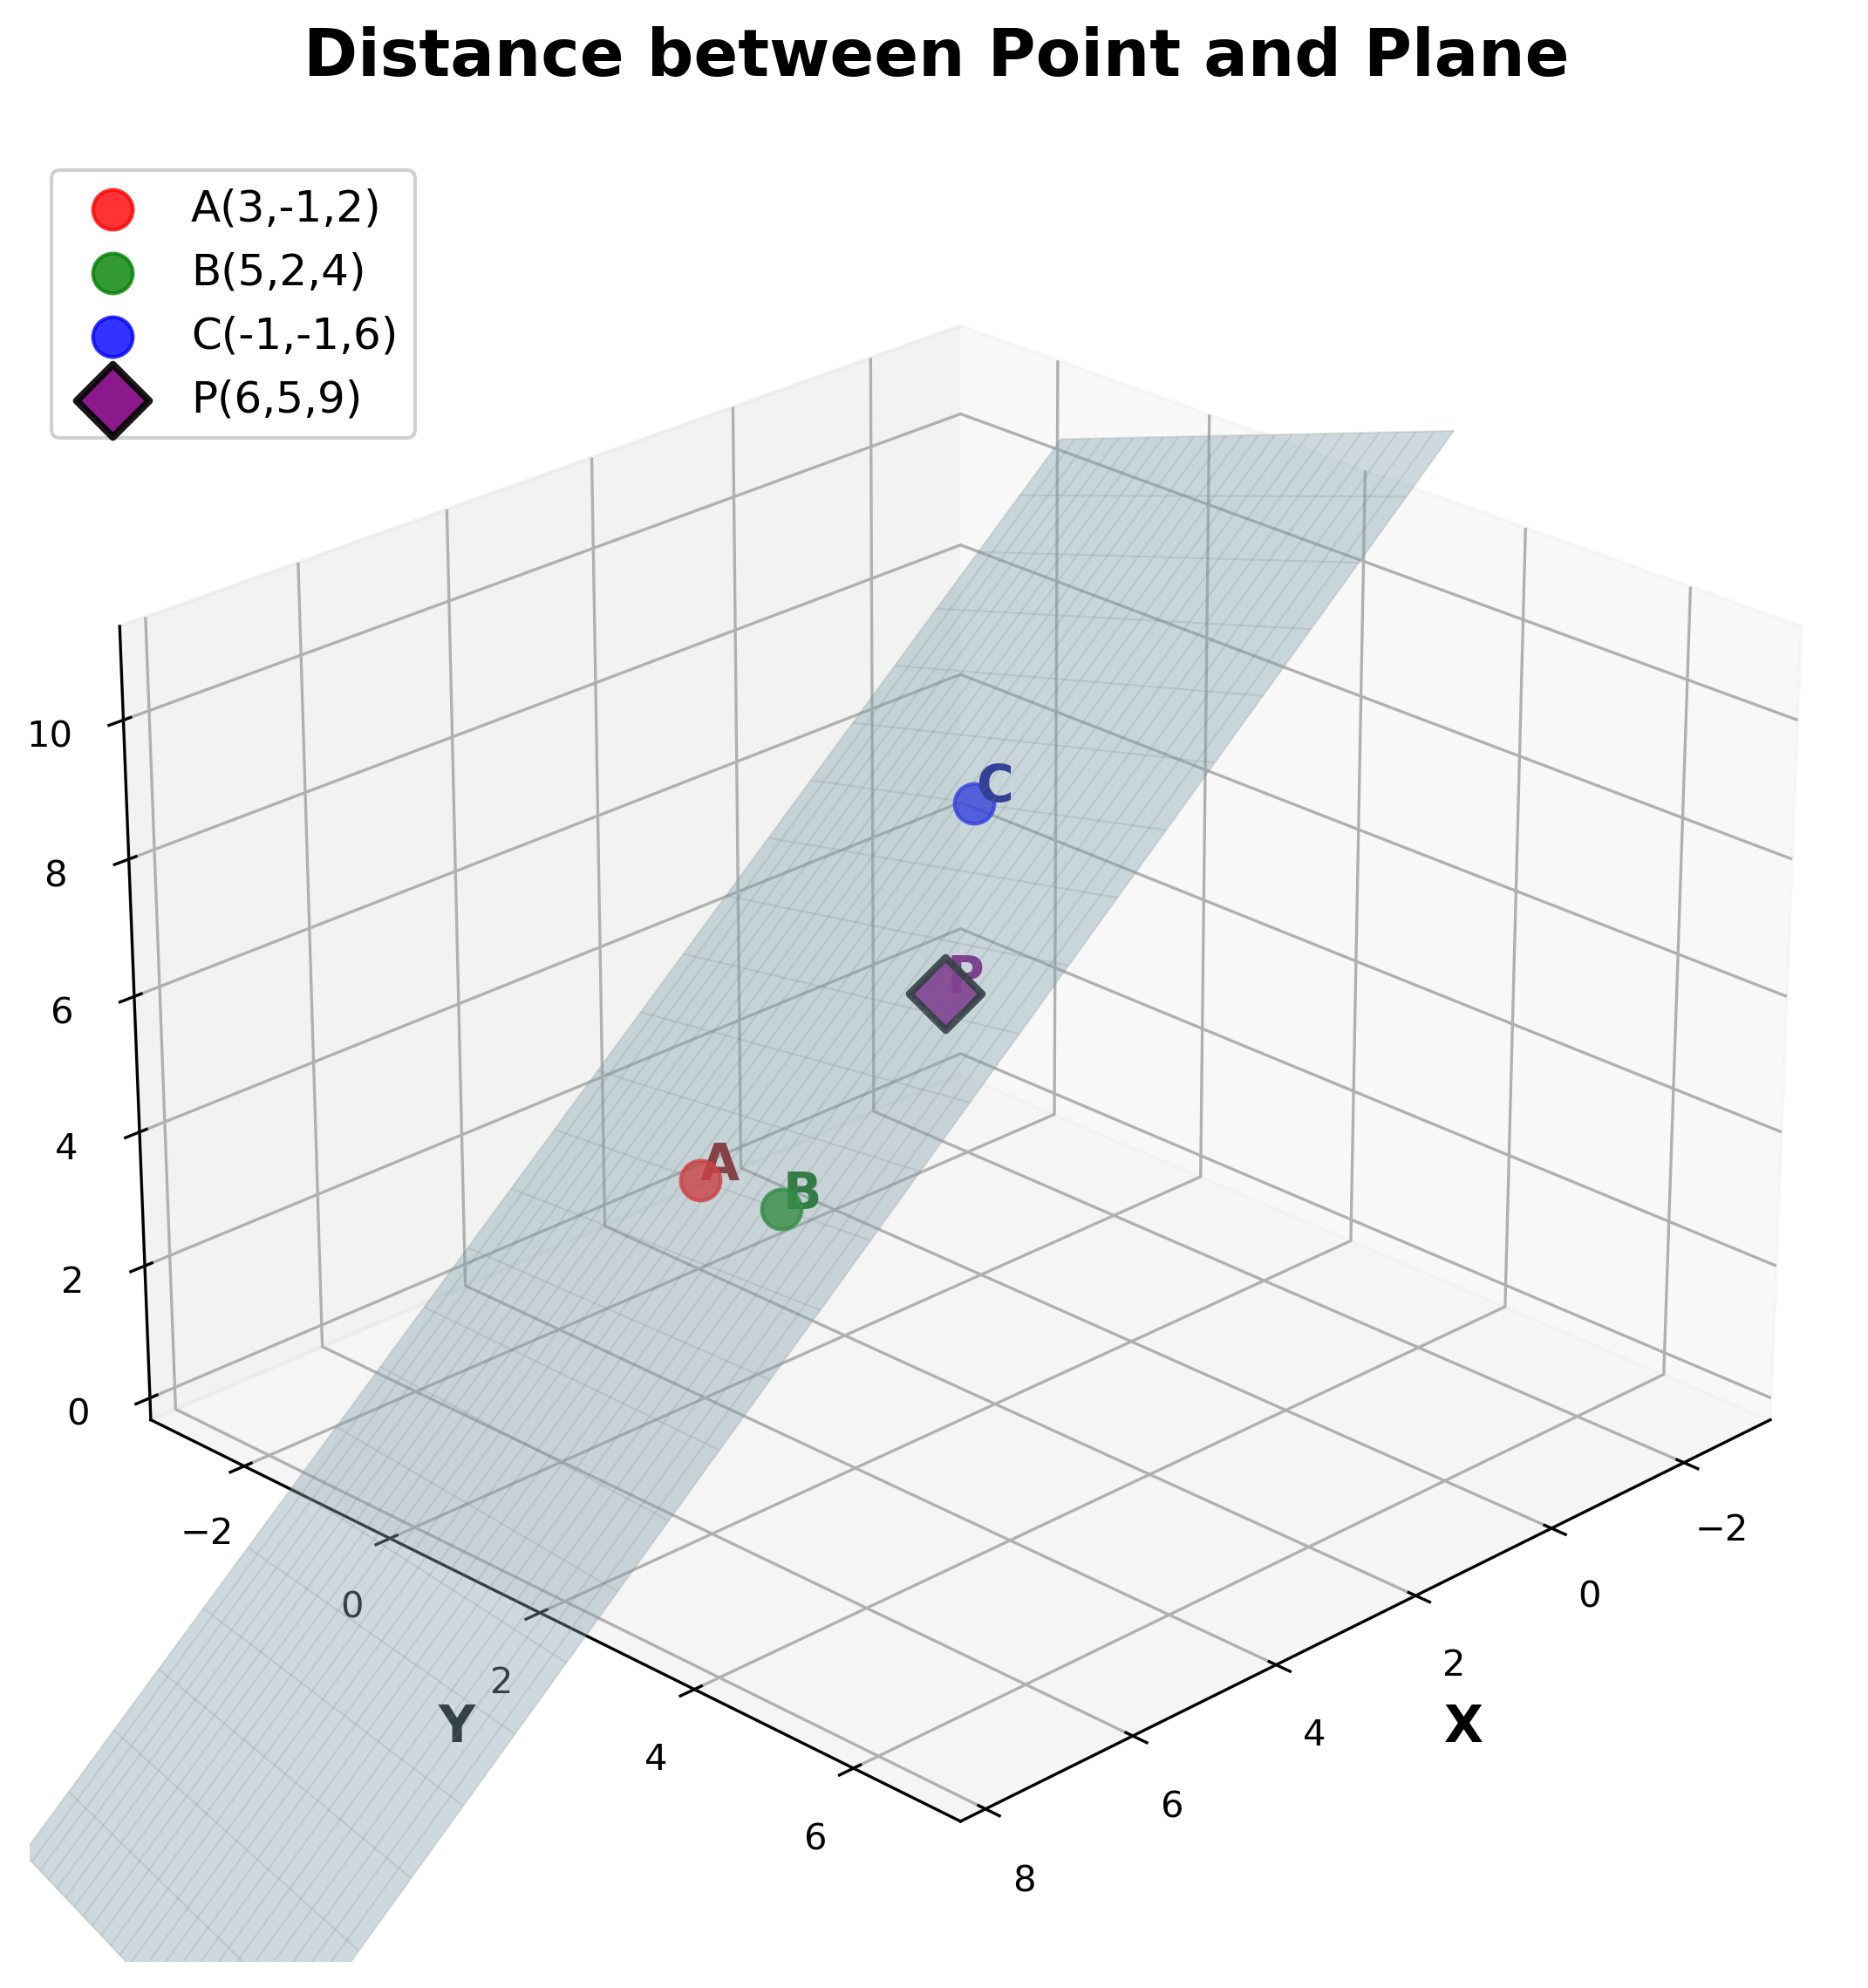
\includegraphics[width=\columnwidth, height=0.8\textheight, keepaspectratio]{figs/fig1.png}
    \label{fig:Beamer/figs/fig1.png}
\end{frame}


\end{document}